% Options for packages loaded elsewhere
\PassOptionsToPackage{unicode}{hyperref}
\PassOptionsToPackage{hyphens}{url}
%
\documentclass[
  a4paper,
]{article}
\usepackage{amsmath,amssymb}
\usepackage{iftex}
\ifPDFTeX
  \usepackage[T1]{fontenc}
  \usepackage[utf8]{inputenc}
  \usepackage{textcomp} % provide euro and other symbols
\else % if luatex or xetex
  \usepackage{unicode-math} % this also loads fontspec
  \defaultfontfeatures{Scale=MatchLowercase}
  \defaultfontfeatures[\rmfamily]{Ligatures=TeX,Scale=1}
\fi
\usepackage{lmodern}
\ifPDFTeX\else
  % xetex/luatex font selection
\fi
% Use upquote if available, for straight quotes in verbatim environments
\IfFileExists{upquote.sty}{\usepackage{upquote}}{}
\IfFileExists{microtype.sty}{% use microtype if available
  \usepackage[]{microtype}
  \UseMicrotypeSet[protrusion]{basicmath} % disable protrusion for tt fonts
}{}
\makeatletter
\@ifundefined{KOMAClassName}{% if non-KOMA class
  \IfFileExists{parskip.sty}{%
    \usepackage{parskip}
  }{% else
    \setlength{\parindent}{0pt}
    \setlength{\parskip}{6pt plus 2pt minus 1pt}}
}{% if KOMA class
  \KOMAoptions{parskip=half}}
\makeatother
\usepackage{xcolor}
\usepackage[margin=2cm]{geometry}
\usepackage{longtable,booktabs,array}
\usepackage{calc} % for calculating minipage widths
% Correct order of tables after \paragraph or \subparagraph
\usepackage{etoolbox}
\makeatletter
\patchcmd\longtable{\par}{\if@noskipsec\mbox{}\fi\par}{}{}
\makeatother
% Allow footnotes in longtable head/foot
\IfFileExists{footnotehyper.sty}{\usepackage{footnotehyper}}{\usepackage{footnote}}
\makesavenoteenv{longtable}
\usepackage{graphicx}
\makeatletter
\def\maxwidth{\ifdim\Gin@nat@width>\linewidth\linewidth\else\Gin@nat@width\fi}
\def\maxheight{\ifdim\Gin@nat@height>\textheight\textheight\else\Gin@nat@height\fi}
\makeatother
% Scale images if necessary, so that they will not overflow the page
% margins by default, and it is still possible to overwrite the defaults
% using explicit options in \includegraphics[width, height, ...]{}
\setkeys{Gin}{width=\maxwidth,height=\maxheight,keepaspectratio}
% Set default figure placement to htbp
\makeatletter
\def\fps@figure{htbp}
\makeatother
\setlength{\emergencystretch}{3em} % prevent overfull lines
\providecommand{\tightlist}{%
  \setlength{\itemsep}{0pt}\setlength{\parskip}{0pt}}
\setcounter{secnumdepth}{-\maxdimen} % remove section numbering
\ifLuaTeX
  \usepackage{selnolig}  % disable illegal ligatures
\fi
\IfFileExists{bookmark.sty}{\usepackage{bookmark}}{\usepackage{hyperref}}
\IfFileExists{xurl.sty}{\usepackage{xurl}}{} % add URL line breaks if available
\urlstyle{same}
\hypersetup{
  pdftitle={DAMSIC Questions},
  pdfauthor={Thomas Debelle; Sjouke Spijkerman; Robin Geens; Sander Crols},
  hidelinks,
  pdfcreator={LaTeX via pandoc}}

\title{DAMSIC Questions}
\usepackage{etoolbox}
\makeatletter
\providecommand{\subtitle}[1]{% add subtitle to \maketitle
  \apptocmd{\@title}{\par {\large #1 \par}}{}{}
}
\makeatother
\subtitle{\href{https://github.com/Tfloow/Q8_KUL}{An Open-Source
Summary}}
\author{Thomas Debelle \and Sjouke Spijkerman \and Robin
Geens \and Sander Crols}
\date{\today}

\begin{document}
\maketitle

{
\setcounter{tocdepth}{3}
\tableofcontents
}
\hypertarget{recap-of-questions-per-chapter}{%
\section{Recap of questions per
chapter}\label{recap-of-questions-per-chapter}}

\hypertarget{sh}{%
\subsection{S\&H}\label{sh}}

\begin{longtable}[]{@{}lrll@{}}
\toprule\noalign{}
Q & page & Q & page \\
\midrule\noalign{}
\endhead
\bottomrule\noalign{}
\endlastfoot
\textbf{1} & 19 & \textbf{2} & 31 \\
\textbf{3} & 44 & & \\
\end{longtable}

\hypertarget{dac}{%
\subsection{DAC}\label{dac}}

\begin{longtable}[]{@{}lrll@{}}
\toprule\noalign{}
Q & page & Q & page \\
\midrule\noalign{}
\endhead
\bottomrule\noalign{}
\endlastfoot
\textbf{4} & 16-17 & \textbf{5} & 28 \\
\textbf{6} & 36 & & \\
\end{longtable}

\hypertarget{adc}{%
\subsection{ADC}\label{adc}}

\begin{longtable}[]{@{}lrll@{}}
\toprule\noalign{}
Q & page & Q & page \\
\midrule\noalign{}
\endhead
\bottomrule\noalign{}
\endlastfoot
\textbf{7} & 9-11 & \textbf{8} & 38 \\
\textbf{9} & 40-41 & \textbf{10} & 56 \\
\textbf{11} & 63 & \textbf{12} & 71 \\
\textbf{13} & 89 & & \\
\end{longtable}

\hypertarget{sigma---delta}{%
\subsection{\texorpdfstring{\(\Sigma - \Delta\)}{\textbackslash Sigma - \textbackslash Delta}}\label{sigma---delta}}

\begin{longtable}[]{@{}lrll@{}}
\toprule\noalign{}
Q & page & Q & page \\
\midrule\noalign{}
\endhead
\bottomrule\noalign{}
\endlastfoot
\textbf{14} & 35,42,45 & \textbf{15} & 53 \\
\textbf{16} & 11,37,46 & \textbf{17} & 46-48 \\
\textbf{18} & 64-65 & \textbf{19} & 11,37 \\
\textbf{20} & XX & & \\
\end{longtable}

\hypertarget{voltage-ref}{%
\subsection{Voltage ref}\label{voltage-ref}}

\begin{longtable}[]{@{}lrll@{}}
\toprule\noalign{}
Q & page & Q & page \\
\midrule\noalign{}
\endhead
\bottomrule\noalign{}
\endlastfoot
\textbf{21} & 18 & \textbf{22} & 29 \\
\end{longtable}

\hypertarget{oscillator}{%
\subsection{Oscillator}\label{oscillator}}

\begin{longtable}[]{@{}lrll@{}}
\toprule\noalign{}
Q & page & Q & page \\
\midrule\noalign{}
\endhead
\bottomrule\noalign{}
\endlastfoot
\textbf{23} & XX & \textbf{24} & 44 \\
\textbf{25} & XX & \textbf{26} & XX \\
\textbf{27} & 28 & \textbf{28} & 45 \\
\end{longtable}

\hypertarget{tuned-amplifiers}{%
\subsection{Tuned Amplifiers}\label{tuned-amplifiers}}

\begin{longtable}[]{@{}lrll@{}}
\toprule\noalign{}
Q & page & Q & page \\
\midrule\noalign{}
\endhead
\bottomrule\noalign{}
\endlastfoot
\textbf{29} & XX & \textbf{30} & 27 \\
\textbf{31} & 38 & \textbf{32} & XX \\
\end{longtable}

\hypertarget{dcdc}{%
\subsection{DCDC}\label{dcdc}}

\begin{longtable}[]{@{}lrll@{}}
\toprule\noalign{}
Q & page & Q & page \\
\midrule\noalign{}
\endhead
\bottomrule\noalign{}
\endlastfoot
\textbf{33} & 1:23 & \textbf{34} & 1:29 \\
\textbf{35} & 1:48 & \textbf{36} & 2:14 \\
\textbf{37} & 2:34 & & \\
\end{longtable}

\hypertarget{wireline}{%
\subsection{Wireline}\label{wireline}}

\begin{longtable}[]{@{}lrll@{}}
\toprule\noalign{}
Q & page & Q & page \\
\midrule\noalign{}
\endhead
\bottomrule\noalign{}
\endlastfoot
\textbf{38} & XX & \textbf{39} & 16 \\
\textbf{40} & XX & \textbf{41} & XX \\
\textbf{42} & 27 & & \\
\end{longtable}

\hypertarget{optical}{%
\subsection{Optical}\label{optical}}

\begin{longtable}[]{@{}lrll@{}}
\toprule\noalign{}
Q & page & Q & page \\
\midrule\noalign{}
\endhead
\bottomrule\noalign{}
\endlastfoot
\textbf{43} & 30-39 & \textbf{44} & XX \\
\textbf{45} & XX & & \\
\end{longtable}

This section is based on the previous work of \emph{Robin Geens} and
\emph{Sander Crols}. Sjouke and I added new questions and answered them
partially. I used notebook LM on top of already answered questions to
add more informations and verified its output.

\hypertarget{h05e3a---exam-questions}{%
\section{H05E3A - Exam Questions}\label{h05e3a---exam-questions}}

Here is a comprehensive response to your query, drawing on the provided
sources:

\begin{enumerate}
\def\labelenumi{\arabic{enumi}.}
\item
  Describe the pedestal step and a possible solution for the problem.

  \begin{itemize}
  \item
    \textbf{Pedestal Step and Solution:} The \textbf{pedestal step} is a
    non-ideality observed in Sample and Hold (S\&H) circuits, appearing
    as an \textbf{abrupt change in the output voltage (\(V_{out}\))}
    during the transition from the sampling phase to the hold phase.
    This effect is visually represented as a sudden upward or downward
    jump in the \(V_{out}\) waveform at the moment the input signal is
    sampled. It is primarily caused by \textbf{charge injection from the
    channel} and by \textbf{parasitic capacitance between the gate and
    output} from the switch as it turns off, specifically due to the
    switch's drain-capacitance and unintended coupling.
  \item
    A possible solution for pedestal step compensation involves using
    \textbf{half-sized dummy switches}. These dummy switches are
    designed to absorb the charge from the main switch, thereby reducing
    the unwanted pedestal step. For this method to work effectively, the
    charge must split approximately 50\% between the main and dummy
    switches. However, the success of this compensation technique is
    critically dependent on the \textbf{careful timing of clock edges}.
    If there are unequal impedances on the left and right sides of the
    main switch, or if clock edges are too fast, it can lead to an
    unequal charge split, which will diminish the effectiveness of the
    compensation. Therefore, ensuring that the \textbf{impedances are as
    equal as possible} is crucial for optimal compensation.
  \end{itemize}
\item
  Discuss the need for bootstrapped switches in switched-capacitor
  circuits.

  \begin{itemize}
  \tightlist
  \item
    The main issue is the fact that \(R_{on} \propto 1/V_{gs}\). So by
    changing the input voltage we change the RC time constant and so it
    creates \textbf{DISTORTION} which is highly unwanted in TH circuits.
    Solution --\textgreater{} Keep it constant using
    \textbf{bootstrapping} aka keep a constant \(V_{gs}\).
  \item
    So we need to keep \(V_{gs}\) high to avoid any saturation. The
    higher the Vgs the smaller the R\_on resistance. We first need to do
    a hold phase on the cap to charge it up to Vdd then in the track
    phase that input voltage is added on top of the cap.
  \item
    Challenges: make sure the body diodes do not open which will result
    in current to substrate, charge lost and latch-up !
  \item
    \textbf{Need for Bootstrapped Switches in Switched-Capacitor
    Circuits:} Bootstrapped switches are important components in
    switched-capacitor (SC) circuits, particularly when \textbf{high
    accuracy} is required. In the context of Delta-Sigma converters, for
    example, they are specifically utilized \textbf{at high accuracies}
    to mitigate the effects of \textbf{clock feedthrough}.
  \end{itemize}
\item
  Discuss offset and noise in the flip-around T/H circuit.

  \begin{itemize}
  \item
    With a regular T\&H circuit, the signal transfer function should be
    1. This means that the sampling capacitor should be equal to the
    feedback capacitor. This results in a feedback factor of 1/2, so a
    closed loop gain of two.
  \item
    An alternative is the flip-around T\&H, which uses no feedback
    capacitor. During both phases, the opamp is in unity gain feedback.
    The offset and low frequency noise are cancelled out, because they
    affect both the V\_C\_hold and the output voltage. The high
    frequency noise is amplified by a factor of two.
  \item
    The offset voltage cancels out because the opamp creates its own
    virtual ground in both phases. Noise transfer function from opamp
    input node to output. The sampled thermal noise on C\_hold is still
    present.
  \item
    \begin{figure}
    \centering
    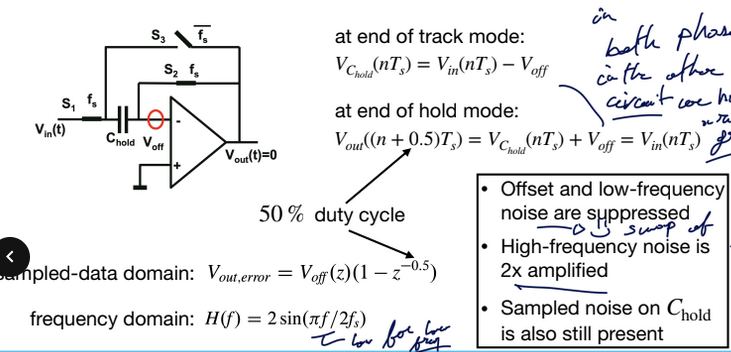
\includegraphics[width=0.75\textwidth,height=\textheight]{image.png}
    \caption{Equations for Flip around}
    \end{figure}
  \end{itemize}
\item
  Discuss the effect of the impedance variation in a resistor ladder in
  resistive DACs

  \begin{itemize}
  \item
    \textbf{Effect of Impedance Variation in Resistor Ladder DACs:} In
    resistive Digital-to-Analog Converters (DACs) employing a resistor
    ladder, the output impedance exhibits a significant variation with
    the input code. This variation is characterized as a
    \textbf{parabolic function}. The equivalent resistance
    (\(R_{eq}(m)\)) can be calculated using the formula
    \(R_{eq}(m) = \frac{m(2^N - m)}{2^{N+1}} R_{tot}\), where \(m\) is
    the digital input code and \(2^N\) is the total number of resistors.
    The maximum equivalent resistance, equal to \(0.25 \cdot R_{tot}\),
    occurs at the midpoint of the digital range.
  \item
    This \textbf{parabolic variation of impedance} has several
    detrimental effects on the DAC's performance:

    \begin{itemize}
    \tightlist
    \item
      It leads to \textbf{signal-dependent current delivery}, meaning
      the current supplied to the load changes non-linearly with the
      input signal. In other terms \textbf{DISTORTION}
    \item
      For a fixed capacitive load, the \textbf{time constant becomes
      signal-dependent}, which affects the settling behavior of the DAC
      output.
    \item
      Collectively, these signal-dependent characteristics introduce
      \textbf{distortion at high frequencies}, degrading the overall
      linearity and dynamic performance of the DAC.
    \end{itemize}
  \end{itemize}
\item
  Discuss the common-centroid layout in the framework of
  current-steering DACs.

  \begin{itemize}
  \tightlist
  \item
    Current steering DAC can be unary or binary. Unary are preferred for
    MSB to avoid big current switch off and on and binary for LSB.
  \item
    Current steering DACs (unary) are very sensitive to mismatches.
    Instead of using matrix decoding, where all sources are placed
    sequentially (according to bit order) in a grid, issue:

    \begin{itemize}
    \tightlist
    \item
      Doping, oxide thickness not constant
    \item
      PSS drop
    \item
      Clock timing
    \item
      Temperature
    \end{itemize}
  \item
    they can be placed according to a common-centroid layout. This
    layout is symmetrical in both dimensions. \textbf{Any linear
    gradient in the production process is cancelled} out by the fact
    that two opposing sources are used (vertical, horizontal and slant).
    The addressing of the sources is less straightforward than with
    matrix decoding.
  \item
    To go even further, every current cell can be subdivided and
    distributed across the array with some \(Q^2\) schemes which improve
    reliability against second order effect.
  \end{itemize}
\item
  Describe the problem of stray capacitances in the design of capacitive
  DACs.

  \begin{itemize}
  \tightlist
  \item
    \textbf{Problem of Stray Capacitances in Capacitive DACs:} Stray
    capacitors are capacitance from the switches right next to the
    (binary scaled) capacitors. The stray capacitor at the left poses no
    problem (not added to output). The charge of the right one is added
    to the feedback capacitor, which means that the total charge
    transferred is no longer correct. The problem can be solved by using
    four switches per capacitor instead of two.
  \item
    In the charge phase, the first stray cap is charged but not the
    right one. The trick in the transfer phase is that the charged left
    cap will have both inputs connected to the same Vref- so it will
    discharge onto this. Thanks to the virtual ground of the opamp, the
    right cap will not be charged making the error 0.
  \item
    Right stray is never charged (thanks to virtual ground of the AMP)
    and left one will charge and discharge on itself
  \end{itemize}
\item
  What limits the regeneration in a latch-based comparator, and how can
  it be improved?

  \begin{itemize}
  \item
    Comparators are difficult blocks as we need \textbf{High BW, high
    AMP, High Accuracy, Wide range, Low power} so latch helps with it
    thanks to a feedback loop but we need a David Goliath latch to still
    be able to change the value on it. Latch is better than cascade of
    amp as cascading amp is \textbf{SLOWWWWW} + Memory effect.
  \item
    2 phase latch with first pre-amp and then latch behavior.
  \item
    \textbf{Limits to Regeneration in Latch-Based Comparators and
    Improvements:} In a latch-based comparator, the regeneration
    process, where a small input difference is amplified to a full
    digital output, is characterized by an exponential growth of the
    differential voltage \(V(t)\) across the latch outputs, given by
    \(V(t) = \alpha V_{LSB} e^{+t/\tau}\). The regeneration speed is
    fundamentally determined by the \textbf{time constant
    \(\tau = C/g_{m,l}\)}, where \(C\) is the parasitic capacitance at
    the output nodes and \(g_{m,l}\) is the transconductance of the
    latch's gain stage. Pre amp --\textgreater{}
    \(A_{pre} = \frac{g_{min}}{C} T_{pre}\)
  \item
    The regeneration in a latch-based comparator is limited by three
    regimes based on the input differential voltage (\(\Delta V_{in}\)):

    \begin{itemize}
    \tightlist
    \item
      \textbf{High \(\Delta V_{in}\)}: The regeneration time is limited
      by the inherent \textbf{propagation delay} of the latch circuit.
      --\textgreater{} Tech constant max speed
    \item
      \textbf{Medium \(\Delta V_{in}\)}: The comparator operates within
      the \textbf{exponential regime}, where the signal grows
      exponentially. --\textgreater{} Take a bit of time to get the
      result \(\tau \approx 10 ps\).
    \item
      \textbf{Small \(\Delta V_{in}\)}: In this critical regime,
      \textbf{noise dominates the input}, leading to potential errors in
      the decision-making process. This is closely related to the
      phenomenon of \textbf{metastability}, where the comparator fails
      to produce a stable output within the required time, resulting in
      an ambiguous output. Metastability can lead to conversion errors
      in Analog-to-Digital Converters (ADCs).
    \end{itemize}
  \item
    To improve regeneration performance and mitigate metastability
    errors:

    \begin{itemize}
    \tightlist
    \item
      One can \textbf{reduce the effective number of bits (N)} in the
      converter, or conversely, \textbf{increase the sampling period
      (\(T_s\))}, which effectively reduces the operating speed.
      --\textgreater{} longer Pre-amp stage to avoid the small
      \(\Delta V_{in}\).
    \item
      Another approach is to \textbf{reduce the time constant \(\tau\)}.
      This can be achieved by decreasing the parasitic capacitance \(C\)
      or increasing the transconductance \(g_{m,l}\) of the latch (so
      higher power consumption, wider NMOS, weak inversion).
    \item
      While metastability is a critical issue for general comparators,
      in Delta-Sigma (\(\Delta\Sigma\)) converters, it is considered
      \textbf{``not an issue''} for the comparator itself because any
      comparator error will be shaped and subsequently filtered.
      However, it is essential to ensure that the digital bit fed to the
      decimation filter is the same as the one fed to the DAC, which
      typically requires placing a \textbf{synchronization latch}.
    \end{itemize}
  \end{itemize}
\item
  How can averaging improve the performance of a flash ADC?

  \begin{itemize}
  \item
    A flash Analog-to-Digital Converter (ADC) utilizes \(2^N-1\)
    comparators to convert an analog input into an N-bit digital word. A
    major non-ideality in flash ADCs is \textbf{comparator offset},
    which results in non-ideal thresholds and contributes to
    differential non-linearity (DNL) errors.
  \item
    While direct ``averaging'' of multiple comparator outputs for
    improved resolution or linearity is not explicitly described, the
    following related techniques are mentioned that contribute to better
    performance:

    \begin{itemize}
    \tightlist
    \item
      \textbf{Auto-zeroing schemes}: These techniques are employed to
      \textbf{cancel comparator offset} and suppress both offset and
      low-frequency noise within individual comparators. This can be
      seen as a form of ``temporal averaging'' or correction within each
      comparator.
    \item
      \textbf{Comparator with Offset Cancellation}: An approach for
      open-loop comparator offset cancellation involves selecting a
      subset (e.g., ``four-out-of-eight minimally sized input pairs'')
      from multiple input pairs. While not explicitly stated as
      averaging their outputs, this selection process aims to achieve a
      more ideal performance by potentially averaging out random offsets
      across a pool of devices.
    \item
      \textbf{Majority voting}: In the context of Successive
      Approximation Register (SAR) ADCs, it's mentioned that
      \textbf{majority voting} can be used to mitigate
      \textbf{comparator noise}. While stated for SAR ADCs, the
      principle of using multiple decisions to reduce noise and errors
      could conceptually be applied to other ADC architectures like
      flash ADCs if multiple comparator outputs are available and
      processed.
    \end{itemize}
  \item
    Offset of the comparators in a flash ADC can cause linearity
    problems and lead to DNL/INL. The effect of offset can be reduced by
    coupling the comparators so that multiple input pairs are used for
    every decision. This is done with resistive coupling, so that
    neighboring decisions influence each other. This helps because the
    signals at the outputs op the comparators add up linearly, but the
    offsets will add up with root mean square. The overall
    signal-to-offset ratio will thus increase. The comparator will
    `appear much larger'.
  \item
    More area needed, more power consumption.
  \end{itemize}
\item
  Discuss the folding technique, its advantages, and challenges.

  \begin{itemize}
  \item
    In a folding circuit, multiple input pairs are cross coupled to
    `fold' the linear input voltage of a regular comparator. This
    reduces the range, so less comparators are needed to convert the
    output of the folding circuit to bits. The conversion is divided
    into a coarse part (the folding itself, pre-processing) and a fine
    part (flash conversion of the folding output). This reduces the
    amount of input pairs: \(2^3 + 2^5\) instead of \(2^8\). One input
    pair of the folding circuit will be active (other ones saturated)
    and which pair will determine the MSB's.
  \item
    The desired transfer curve of the folding circuit contains
    non-linearities in the peaks (\textbf{distortion at crossover
    points}). It is not possible to realize this in practice, so when
    the input voltage is in this range, it will be distorted. A solution
    to this is by using double the amount of input pairs in two folding
    circuits. Then we either \textbf{interpolate} those two folding
    circuits or take the one that is working in its \textbf{linear}
    region.
  \item
    There is some delay, and we need some good amplifier to realize the
    fine conversion.
  \item
    \begin{figure}
    \centering
    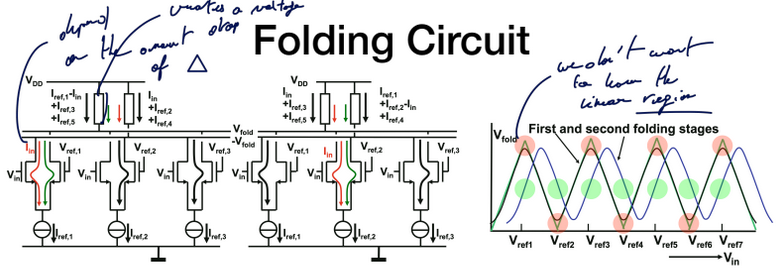
\includegraphics[width=0.75\textwidth,height=\textheight]{image-1.png}
    \caption{Folding circuits}
    \end{figure}
  \end{itemize}
\item
  \textbf{Advantages and Disadvantages of a 1.5-bit Pipeline Converter
  Compared to a 1-bit Pipeline Converter:}

  Pipeline converters break down the analog-to-digital conversion into
  multiple stages, each processing a certain number of bits. The
  comparison between 1-bit and 1.5-bit stages primarily revolves around
  trade-offs in speed, complexity, and accuracy.

  \textbf{1-bit Pipeline Converter:}

  \begin{itemize}
  \tightlist
  \item
    Straight forward, check if value is above or below \(V_{ref}/2\),
    multiply by 2, next stage, repeat. If an error before, will ripple
    through the chain.
  \item
    \textbf{Advantages:}

    \begin{itemize}
    \tightlist
    \item
      \textbf{Maximum speed}: With its subrange limited to a single bit,
      it typically uses an amplifier with a 2x gain, which can achieve
      high conversion speeds.
    \item
      \textbf{Intrinsic linearity}: The 1-bit DAC in its feedback loop
      is inherently linear, contributing to the overall intrinsic N-bit
      precision of the converter. A 1-bit DAC is always perfectly
      linear, and time-domain converters leverage this for excellent
      linearity.
    \item
      \textbf{Simplicity}: Requires only a single comparator for its
      analog-to-digital conversion within each stage.
    \item
      The basic building block is a Multiplying Digital-to-Analog
      Converter (MDAC).
    \end{itemize}
  \item
    \textbf{Disadvantages:}

    \begin{itemize}
    \tightlist
    \item
      \textbf{Delay}: The full digital value is available after N+3
      clock periods, as each stage processes one bit sequentially. This
      delay, while exchanged for speed, can be problematic in feedback
      loops.
    \item
      Potentially more stages required for a given resolution compared
      to multi-bit stages, which could increase overall complexity and
      power (though per-stage power is low).
    \item
      \textbf{Good and accurate settling in all the stages}
    \end{itemize}
  \end{itemize}

  \textbf{1.5-bit Pipeline Converter (a type of Multi-Bit MDAC Pipeline
  Converter):}

  \begin{itemize}
  \item
    Will have \(\pm V_{ref}/4\) if 2 positive decision, subtract
    \(V_{ref}\), 2 negative add \(V_{ref}\) else do nothing.
  \item
    \begin{figure}
    \centering
    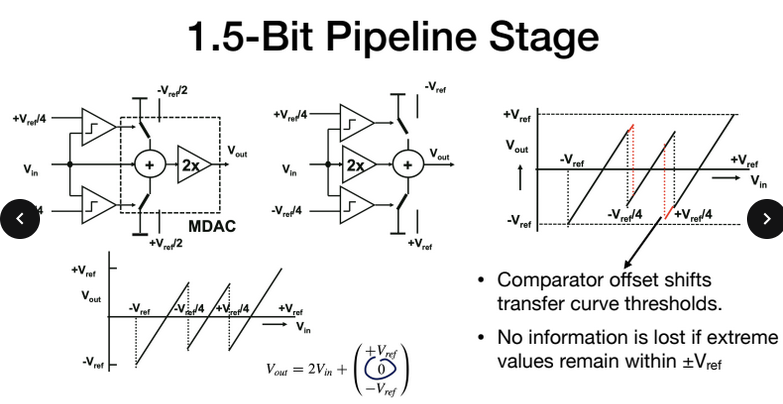
\includegraphics[width=0.75\textwidth,height=\textheight]{image-2.png}
    \caption{Offset doesn't impact precision since added reliability}
    \end{figure}
  \item
    \begin{figure}
    \centering
    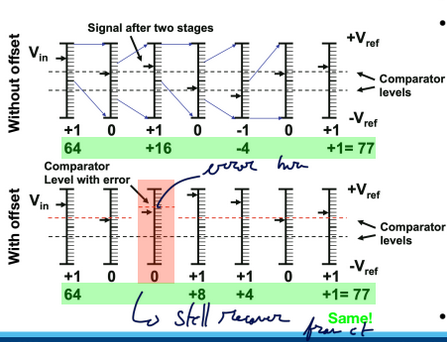
\includegraphics[width=0.75\textwidth,height=\textheight]{image-3.png}
    \caption{Redundancy}
    \end{figure}
  \item
    \textbf{Advantages:}

    \begin{itemize}
    \tightlist
    \item
      \textbf{More aggressive stage-scaling}: By processing more than
      one bit per stage (e.g., 1.5 bits, 2.5-4 bits), these converters
      allow for a reduction in the total number of stages required for a
      given resolution. This can lead to more compact designs.
    \item
      \textbf{Error Correction Margin}: Having more levels per stage
      (e.g., six segments for 2.5 bits) provides a margin to correct
      errors that might occur in the comparators.
    \item
      \textbf{Higher Overall Performance}: Can achieve higher effective
      number of bits (ENOB) at comparable or higher sample rates
      compared to purely 1-bit per stage designs, as seen in examples
      where 2.5-bit stages are used at the front-end followed by 1.5-bit
      stages.
    \end{itemize}
  \item
    \textbf{Disadvantages/Challenges:}

    \begin{itemize}
    \tightlist
    \item
      \textbf{Slower amplifier settling}: Due to the higher gain
      required in multi-bit stages (e.g., 4x or 8x gain), the amplifiers
      need more time to settle accurately.
    \item
      \textbf{More complex DACs}: The first stage requires a multi-level
      DAC (e.g., a five-level DAC for a 2.5-bit stage) that must
      maintain the \textbf{full accuracy of the entire converter}. This
      multi-bit DAC is a critical component and its non-linearity due to
      mismatch can be a significant problem.
    \item
      \textbf{Increased Complexity for DAC Linearity}: Mismatch in
      multi-bit DACs can generate non-linearity errors. Techniques like
      \textbf{Data Weighted Averaging (DWA)} are used to make these
      errors noise-like so they can be filtered by oversampling,
      resulting in much lower harmonic distortion. This adds complexity
      to the digital processing.
    \item
      Offset is not removed and we hope that the redundancy will help.
      Or high-freq noise amplified
    \end{itemize}
  \end{itemize}
\item
  Opamp Sharing Technique in Pipeline Converters

  The opamp sharing technique in pipeline converters allows a single
  operational amplifier (opamp) to be used in two subsequent stages of
  the converter. This approach is implemented by adapting the
  Multiply-Digital-to-Analog Converter (MDAC) structure to share the
  opamp between channels.

  The main advantage of this technique is a \textbf{significant
  reduction in power consumption, often by a factor of 2x}. However,
  this comes with certain trade-offs:

  \begin{itemize}
  \tightlist
  \item
    \textbf{Offset voltage is not compensated}. No auto-zeroing
    technique
  \item
    It can introduce a \textbf{memory effect between subsequent
    samples}.
  \item
    It is only feasible if the opamp is not required to create a virtual
    ground during its operation.
  \end{itemize}
\item
  Differences Between Top-Plate and Bottom-Plate Sampling

  In the context of charge-redistribution converters, sampling involves
  connecting the input signal to a capacitor bank. The sources describe
  two primary methods:

  \textbf{Top-Plate Sampling:}

  \begin{itemize}
  \tightlist
  \item
    \textbf{No attenuation of the sampled voltage} occurs.
  \item
    However, it causes an \textbf{attenuation of the reference voltage}.
  \item
    The Most Significant Bit (MSB) can be determined directly after
    sampling.
  \end{itemize}

  Problematic for high accuracy as not same attenuation between ref and
  input but faster.

  \textbf{Bottom-Plate Sampling:}

  \begin{itemize}
  \tightlist
  \item
    This method results in \textbf{the same attenuation for both the
    input and reference voltages}.
  \item
    A key advantage is that the \textbf{input voltage range can be made
    equal to the reference voltage range}.
  \item
    A common-mode voltage (VCM) is employed to maintain the comparator
    input at the desired level.
  \end{itemize}

  Trickier setup with the common mode, will be slower but really good
  for high accuracy ADC. We have a precharge phase.
\item
  Comparison of Dual-Slope Converter with a Straightforward Slope
  Converter

  Both dual-slope converters and straightforward slope (or linear
  approximation/counting) converters belong to the category of linear
  search converters. They differ significantly in their operation and
  characteristics:

  \textbf{Straightforward Slope (Linear Approximation/Counting)
  Converter:}

  \begin{itemize}
  \tightlist
  \item
    \textbf{Operation Principle:} The converter uses a counter to
    linearly increase the output of a Digital-to-Analog Converter (DAC).
    A comparator continuously compares this increasing DAC output
    (V\_DAC) with the sampled input signal (V\_signal). Once V\_DAC
    exceeds V\_signal, the comparator toggles, and the current counter
    value is stored as the digital output; the counter is then reset.
  \item
    \textbf{Conversion Time:} The output is ready after \textbf{\(2^N\)
    clock cycles}, where N is the number of bits. This is considerably
    slower compared to flash (1 clock cycle) or pipeline (N clock
    cycles) converters.
  \item
    \textbf{Input Handling:} An input Sample \& Hold (S/H) circuit is
    required to keep the input signal constant during the conversion
    period.
  \item
    \textbf{Offset:} The comparator offset can be added to the digital
    output code. Usually we first convert known ref signal then measure
    actual signal and subtract both of them.
  \item
    \textbf{Applications:} Often used in applications like image sensor
    readouts, where one ADC per column shares a DAC and counter. Small
    transistors in comparators in such applications can lead to offset
    and 1/f noise, necessitating correlated double sampling to measure a
    known reference and the signal, then digitally subtract the values.
    Can be used as a tracking converter with minimum changes.
  \end{itemize}

  \textbf{Dual-Slope Converter:}

  \begin{itemize}
  \tightlist
  \item
    \textbf{Operation Principle:} This converter operates in two
    distinct phases:

    \begin{enumerate}
    \def\labelenumii{\arabic{enumii}.}
    \tightlist
    \item
      \textbf{Integration Phase:} The input signal is integrated for a
      fixed sample period.
    \item
      \textbf{Discharge Phase:} The integrated capacitor is then
      discharged by a fixed reference current. The time taken for
      discharge is proportional to the integrated input signal, and this
      time is measured to determine the digital output.
    \end{enumerate}
  \item
    \textbf{Conversion Time:} The conversion time is typically
    \textbf{\((2 \cdot 2^N)/f_s\)}, making it suitable for slowly
    varying input signals.
  \item
    \textbf{Offset Cancellation:} A significant advantage is that
    \textbf{offsets are cancelled} due to the two-phase operation, as
    the same integrator and comparator are used for both the input
    signal and the reference current. This is an example of a
    ``zero-crossing method'' where linearity is primarily required
    around the zero level.
  \item
    \textbf{Linearity:} Linearity is only required around the zero level
    for the comparison, as the unknown signal is determined by comparing
    it to an equivalent signal from the DAC.
  \end{itemize}
\item
  Why are 1st order or higher-order single-loop sigma-delta topologies
  not advised?

  Higher order loops are not inherently stable. Every low pass filter
  adds a ninety-degree phase shift which means that anything above
  second order can become unstable. Need a precise \(b_1\) to counter
  balance and stabilize the loop.

  \begin{figure}
  \centering
  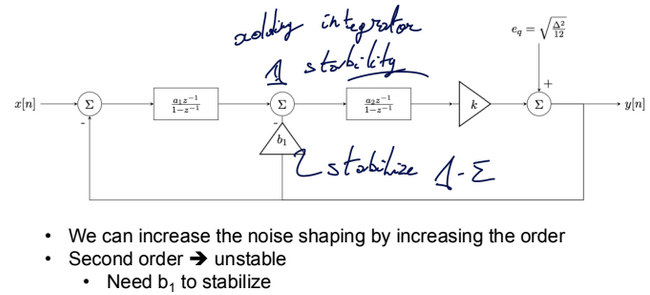
\includegraphics[width=0.75\textwidth,height=\textheight]{image-4.png}
  \caption{Second order issue}
  \end{figure}

  Stability can be shown with the limit cycle and we see that it
  shouldn't spiral out. If it spirals out, it will get limited by PSS
  and so create \textbf{distortion}.

  In the derivation of the sigma delta converter, we assumed a white
  noise distribution. This assumption is not correct for first order
  \(\Sigma - \Delta\) converters. There is a lot of clicking and
  \textbf{pattern noise} because of deterministic quantization noise.
  This creates a \textbf{dead zone} in the DC function that spans 2 - 3
  bits. Noise shaping doesn't work anymore

  In higher order topologies, the intermediate signals must become
  smaller to limit signal swing after the next integrator. This means
  that the SNR ratio is inherently reduced. (not a problem in
  feedforward topologies) Furthermore, higher order topologies are
  unstable for certain combinations of filter coefficients. This makes
  the implementation very difficult. Truly dependent of the
  implementation and precision of the weights.

  If there is an interest in increasing the order of a
  \(\Sigma - \Delta\) converter, MASH converters are advised that
  cascade multiple lower order modulators and will decorrelate noise
  from its signal without becoming more unstable(n 1st order loops,
  instead of 1 n\^{}th order loop)
\item
  Explain the principle of data-weighted averaging.

  \textbf{Data-Weighted Averaging (DWA)} is a noise shaping technique
  used in oversampling applications. Its main idea is to
  \textbf{modulate the error}. In a multi-bit Digital-to-Analog
  Converter (DAC) within the feedback path of a Delta-Sigma converter,
  mismatch between DAC elements can generate non-linearity errors.

  While simple offset errors can be easily ``chopped'' (a modulation
  technique) and filtered by the zeros in the decimation filter, the
  errors caused by mismatch in multi-bit DACs are signal-dependent,
  leading to distortion. DWA addresses this problem by making these
  signal-dependent errors \textbf{noise-like}, allowing the oversampling
  process to filter them off.

  DWA will cycle through the cells and so will smooth out the error, it
  will transform the distortion into an equivalent white noise pattern.
  It is the same idea as for SD
\item
  Discuss the advantages and disadvantages of single-bit and multi-bit
  sigma-delta converters.

  Using a higher order (stability problems with classical topology so
  use cascade) or using multi-bit DACs in the feedback path.

  \textbf{Single-bit Sigma-Delta Converters:}

  \begin{itemize}
  \tightlist
  \item
    \textbf{Advantage:} A 1-bit DAC (Digital-to-Analog Converter) is
    \textbf{inherently linear}. This eliminates non-linearity errors
    that can arise from element mismatch in multi-bit DACs in the
    feedback path.
  \end{itemize}

  \textbf{Multi-bit Sigma-Delta Converters:}

  \begin{itemize}
  \tightlist
  \item
    \textbf{Advantages:} indicating high performance in these areas,
    especially compared to ``Single Loop'' and ``Cascade''. Multi-bit
    converters, particularly Delta-Sigma converters with low
    Over-Sampling Ratio (OSR), are considered suitable for
    ``High-Resolution High-Speed AD converters''.
  \item
    \textbf{Disadvantage:} The main problem with multi-bit Delta-Sigma
    converters is the \textbf{linearity of the multi-bit DAC in the
    feedback path}. Mismatch between the individual DAC elements will
    generate non-linearity errors. Techniques like Data-Weighted
    Averaging (DWA) are employed to mitigate this issue by making the
    signal-dependent error noise-like so it can be filtered out by
    oversampling. Typically we need a DAC in the return which was not
    needed in 1-bit ADC !
  \item
    \textbf{Solutions:} can use chopping, dynamic element matching.
    Offset is okay if we can one time add it then remove it so on
    average it is null and can be seen as a noise that the OSR nature of
    SD will take care of.
  \end{itemize}
\item
  Explain limit cycles in delta-sigma converters. Why do we need them
  but why do we want them to be random?

  \begin{itemize}
  \item
    \textbf{The problem:} If there is \textbf{no noise} and the input
    signal to a Delta-Sigma converter is a ``static'' or near-DC signal,
    the ``white noise approximation'' for quantization does not hold up,
    and oversampling alone does not help in noise reduction. In such
    cases, the quantization error might become correlated with the
    input, leading to \textbf{predictable, undesired tones or patterns
    in the output spectrum} instead of spread-out noise. This is what is
    typically referred to as \textbf{limit cycles or idle tones}. Also
    they should be stable and non-repetitive to avoid distortion.
  \item
    \textbf{The solution/why we want them random:} If they are not
    random, they will lead to a 2-3 bits LSB blindness. To overcome this
    limitation, the system needs to ``store the error and add it to the
    previous sample''. More broadly, the idea is to ensure that the
    quantization error is random and wideband, so it can be shaped and
    filtered.
  \end{itemize}
\item
  Describe CIC decimation filters and their latency when used in an
  incremental converter.

  A CIC (Cascaded Integrator-Comb) filter is a simple (only
  additions/subtractions!) and efficient decimation filter used in SD
  converters. It consists of integrator stages followed by comb
  (differentiator) stages and acts like a low-pass sinc filter to remove
  out-of-band quantization noise while reducing the sample rate.
  \[T_{\text{avg}} = \left( \frac{1}{M} \frac{1 - z^{-M}}{1 - z^{-1}} \right)^{n} \\ = \frac{1}{M} \left( \frac{1}{1 - z^{-1}} \right)^{n} \left( \frac{1 - z^{-M}}{1} \right)^{n}\]

  \begin{figure}
  \centering
  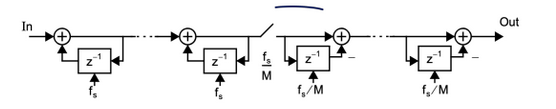
\includegraphics[width=0.75\textwidth,height=\textheight]{image-5.png}
  \caption{CIC filter}
  \end{figure}

  In incremental sigma-delta converters, which operate over short
  measurement windows, CIC filters are still used for decimation, but
  their latency matters. The output becomes valid only after the full
  integration and comb operation is complete, resulting in a latency of
  roughly \[ (n+2) \cdot OSR \cdot 2\cdot  T_s=latency \quad [time]\]

  Where n is the number of stages. The factor 2 comes from one cycle for
  integration, and one cycle for differentiation. Per sample an
  integration and decimation is needed. It is based on the sinc function
  which in frequency domain is an ideal brick wall filter. The idea is
  to combinate integrator and differentiator.
\item
  What is the advantage of oversampling sigma-delta techniques for the
  design of the anti-alias filters? What is the difference between
  discrete and continuous time DS converters?
\end{enumerate}

\begin{itemize}
\item
  \textbf{Advantage of oversampling for anti-alias filters:} In
  Delta-Sigma converters, \textbf{oversampling} is a fundamental
  principle that allows the quantization noise to be spread over a wider
  frequency band. This noise is then shaped, meaning it's pushed out of
  the desired signal band. The ``loop filter'' within the Delta-Sigma
  modulator helps in this noise shaping. As a result, the demanding
  requirements on the \textbf{anti-alias filter} are relaxed. For
  example, a \textbf{continuous-time Delta-Sigma converter itself can
  function as an anti-alias filter}, which also helps in saving power.
  This is because the oversampling and noise shaping inherently provide
  significant attenuation for out-of-band signals, reducing the need for
  a steep, high-order external analog anti-alias filter.

  When no oversampling is used, the input signal should not have
  frequencies larger than \(f_s/2\). Otherwise, the higher frequency
  components will be folded on top of the lower ones when the signal is
  sampled, which results in aliasing. This LPF should ideally be a
  perfect brick-wall filter with a cutoff frequency of \(f_s/2\). This
  is not possible to realize in practice.

  With an oversampling converter, the sampling happens at a higher
  frequency than the Nyquist frequency. Frequency components (a bit)
  higher than Nyquist frequency will not result in aliasing. This
  relaxes the requirements of the analog low-pass filter while spreading
  out the noise quantity. The converted digital signal will be down
  sampled to return to the Nyquist frequency, and this might result in
  aliasing if the signal is not properly filtered first. But this
  filtering operation can be done in the digital domain, which is
  easier.

  In continuous-time converters, the loop filter runs continuously using
  resistors, capacitors, and amplifiers. This gives a natural
  anti-aliasing effect without extra filtering stages and saves power,
  but comes with drawbacks: it's more sensitive to clock jitter,
  component variation (like resistor mismatch), and offers less
  flexibility for tuning or reconfiguration.

  \begin{itemize}
  \tightlist
  \item
    \textbf{Difference between discrete and continuous time DS
    converters:}

    \begin{itemize}
    \tightlist
    \item
      The sources implicitly differentiate between discrete and
      continuous-time Delta-Sigma (DS) converters.
    \item
      A \textbf{continuous-time Delta-Sigma converter} has the advantage
      that its loop filter \textbf{can also function as an anti-alias
      filter}, potentially saving power. However, it is susceptible to
      clock jitter, which can add noise, and the use of resistors for
      feedback (to combat jitter) can lead to wide variations over
      different process corners and a less \textbf{flexible
      architecture}.
    \item
      \textbf{CHECK LECTURE CAUSE I AM PRETTY SURE HE SAID SOMETHING}
    \end{itemize}
  \end{itemize}
\end{itemize}

\begin{enumerate}
\def\labelenumi{\arabic{enumi}.}
\setcounter{enumi}{19}
\item
  What happens if, instead of a lowpass filter, a bandpass filter is
  used as noise shaping filter in a sigma-delta ADC?

  If a \textbf{bandpass filter} is used as the noise shaping filter
  (also referred to as the ``loop filter'') in a Delta-Sigma ADC, the
  system becomes a \textbf{bandpass delta-sigma converter}. This means
  that instead of pushing the quantization noise to high frequencies (as
  a low-pass noise shaping filter does), the noise is shaped and moved
  away from a specific central frequency band, concentrating the signal
  within that band. An advantage of this approach is that
  \textbf{demodulation can be done directly on the bitstream in the
  digital domain} using simple operations like multiplication by +1 or
  -1. This implies that a bandpass Delta-Sigma ADC is suitable for
  signals that are already modulated around a carrier frequency,
  removing the need for a separate mixer.

  \begin{figure}
  \centering
  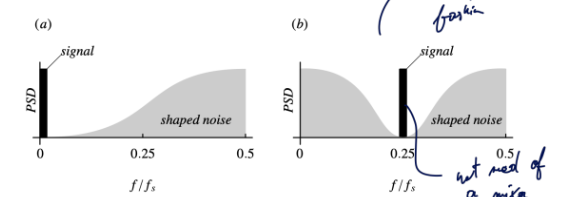
\includegraphics[width=0.75\textwidth,height=\textheight]{image-6.png}
  \caption{Band pass}
  \end{figure}
\item
  Schematic of a Low Voltage Bandgap with Folded Resistors

  \begin{figure}
  \centering
  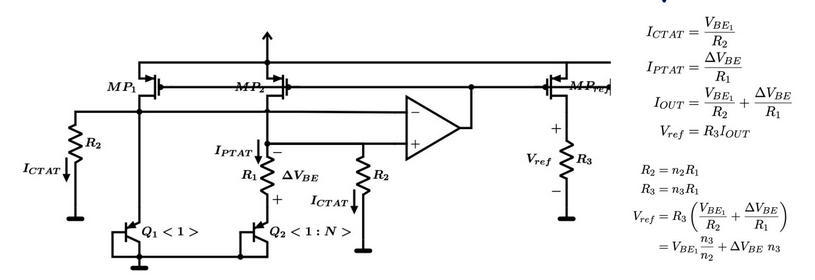
\includegraphics[width=0.75\textwidth,height=\textheight]{image-8.png}
  \caption{Folded resistors low voltage bandgap}
  \end{figure}

  The sources present a schematic for a low voltage bandgap reference
  which incorporates ``folded resistors'' and sums proportional to
  absolute temperature (PTAT) and complementary to absolute temperature
  (CTAT) components in the current domain. This design addresses the
  challenge of implementing a 1.2V silicon bandgap in a 1.2V technology,
  such as 65nm.

  The circuit shown (identified as a ``Static Start-up circuit'' but
  also appearing as the core bandgap circuit) consists of:

  \begin{itemize}
  \tightlist
  \item
    \textbf{Bipolar Junction Transistors (BJTs) Q1 and Q2:} These
    generate the temperature-dependent voltages. Q1 has a scaling factor
    of \texttt{\textless{}1\textgreater{}} and Q2 has a factor of
    \texttt{\textless{}1:\ N\textgreater{}}, indicating that Q2 is N
    times larger than Q1, or that N unit transistors are used for Q2.
    The difference in their base-emitter voltages, \(\Delta V_{BE}\), is
    proportional to absolute temperature (PTAT).
  \item
    \textbf{Resistors R1 and R2:} R1 is used to generate the PTAT
    current. R2 generates a current that is complementary to absolute
    temperature (CTAT), as it is connected in series with Q1, whose
    \(V_{BE}\) exhibits a negative temperature coefficient.
  \item
    \textbf{Operational Amplifier (OpAmp):} The OpAmp forces the voltage
    at its two input terminals to be equal. In this circuit, one input
    is connected to the collector of MP1 and the other to a node between
    R1 and the emitter of Q2.
  \item
    \textbf{PMOS Transistors MP1 and MP2:} These act as current mirrors.
    MP1 mirrors a current derived from Q1 and R2, while MP2 receives
    current from the node where R1, Q2, and the OpAmp's negative input
    connect.
  \end{itemize}

  \textbf{Current Generation and Summation:} The circuit operates by
  generating two primary currents:

  \begin{itemize}
  \tightlist
  \item
    \textbf{\(I_{CTAT}\) (Complementary To Absolute Temperature):} This
    current is defined as \(I_{CTAT} = \frac{V_{BE1}}{R_2}\). Since
    \(V_{BE}\) decreases with increasing temperature, \(I_{CTAT}\) will
    also decrease with increasing temperature.
  \item
    \textbf{\(I_{PTAT}\) (Proportional To Absolute Temperature):} This
    current is defined as \(I_{PTAT} = \frac{\Delta V_{BE}}{R_1}\). The
    difference in base-emitter voltages (\(\Delta V_{BE}\)) between Q1
    and Q2, due to their emitter area ratio, is proportional to absolute
    temperature. Thus, \(I_{PTAT}\) increases with increasing
    temperature.
  \end{itemize}

  The design ``is adding ptat and ctat in the current domain''. The
  total output current, \(I_{OUT}\), is the sum of these two currents:
  \(I_{OUT} = \frac{V_{BE1}}{R_2} + \frac{\Delta V_{BE}}{R_1}\). By
  appropriately sizing R1, R2, and the BJT area ratio (N), these two
  temperature-dependent currents can be made to cancel each other's
  temperature dependency, resulting in a temperature-independent output
  current.

  The ``folding of resistors'' is mentioned as a technique similar to
  that used in folded cascode operational transconductance amplifiers
  (OTAs). This technique can allow the circuit to operate with a lower
  supply voltage (e.g., \(V_{DD} < 1V\) for CMOS bandgaps), as it
  reduces the required voltage headroom by allowing different parts of
  the circuit to operate at different voltage levels without stacking
  them directly.

  Finally, a temperature-independent reference voltage, \(V_{ref}\), is
  generated by passing the stable \(I_{OUT}\) through an additional
  resistor R3: \(V_{ref} = R_3 I_{OUT}\). If R2 and R3 are designed as
  multiples of R1 (i.e., \(R_2 = n_2 R_1\) and \(R_3 = n_3 R_1\)), the
  reference voltage can be expressed as
  \[V_{ref} = V_{BE1} \frac{n_3}{n_2} + \Delta V_{BE} n_3\]
\item
  Why are Voltage References More Accurate than Current References?

  \begin{itemize}
  \item
    \textbf{Voltage References (Vref):} Bandgap voltage references are
    described as being based on a ``physical constant,'' which
    contributes to their high accuracy. The silicon bandgap voltage is
    approximately 1.2V. This inherent physical property provides a
    robust and predictable reference. While factors like matching, ratio
    accuracy, and curvature correction (to linearize temperature
    dependence) are important design considerations, the core reference
    relies on a fundamental material constant. We can match the CTAT
    with the PTAT making it reliable. Moreover, the resistance do not
    really matter, we keep them unit and enhance the matching like this.
  \item
    \textbf{Current References (Iref):} In contrast, current references
    are stated to be ``Based on Vref and R''. The crucial distinction is
    that they have ``No physical parameter'' directly underlying their
    value, leading to ``limited accuracy''. While current references
    also involve considerations such as matching, ratio accuracy, and
    curvature correction, their ultimate stability and accuracy are
    inherently tied to the stability and accuracy of the voltage
    reference they are derived from, as well as the precision of the
    resistor used. Resistive elements can have variations in their sheet
    resistance (e.g., Poly, p+, p-well resistors have absolute
    tolerances of 30\%, 22\%, and 66\% respectively) and temperature
    coefficients (e.g., 0.2, 0.4, and 2 for the temperature exponent
    \(\alpha\) in \(R=R_{300}(T/300)^\alpha\)). These variations can
    directly impact the accuracy of a current reference that relies on
    them. Accuracy of current source can be as low as \(\pm 35 \%\).
  \end{itemize}

  In summary, bandgap voltage references leverage a fundamental and
  stable physical property of silicon, making them inherently more
  accurate. Current references, however, are typically \emph{derived}
  from a voltage reference and a resistor, introducing additional
  dependencies and potential inaccuracies from the resistor's
  characteristics.
\item
  \textbf{Why do we need an amplitude control loop in the design of a
  Xtal oscillator?}

  An amplitude control loop is crucial in the design of a Crystal (Xtal)
  oscillator due to significant variations that can occur during the
  production process. When designing a Xtal oscillator under nominal
  conditions, there can be \textbf{huge variations in production},
  specifically:

  \begin{itemize}
  \tightlist
  \item
    +/- 20\% in capacitance.
  \item
    +/- 20\% in transconductance (gm).
  \end{itemize}

  These production variations can lead to several problematic conditions
  for the oscillator:

  \begin{itemize}
  \tightlist
  \item
    The oscillator may \textbf{fail to start up}.
  \item
    The \textbf{drive power might exceed the rated limits of the
    crystal}, potentially causing lifetime issues for the crystal.
  \end{itemize}

  To mitigate these issues, especially when considering performance
  variations ``over corners'' (referring to different operating
  conditions and manufacturing variations), an amplitude control loop
  must be implemented. This ensures that the \textbf{amplitude is
  regulated}, preventing excessive power consumption and crystal damage
  while guaranteeing reliable startup. Without it, if the
  transconductance (gm) is too high (gm \textgreater{} gm\_opt), more
  power is consumed to compensate for Rs, and if gm exceeds a certain
  critical value (gm \textgreater{} gmA), the amplitude will grow until
  the average gm drops back to gmA, which can lead to \textbf{distortion
  due to non-linear behavior}.
\item
  \textbf{Describe the design of a Pierce oscillator.}

  The sources outline key considerations for designing a \textbf{Crystal
  (Xtal) oscillator}, which commonly refers to a Pierce oscillator
  configuration, as indicated by the typical circuit diagram. The design
  process involves balancing several factors to ensure stable
  oscillation and desired performance.

  \textbf{Key design parameters and considerations:}

  \begin{itemize}
  \tightlist
  \item
    \textbf{Crystal parameters:} Start with the specific parameters of
    the crystal, including its series resonance frequency (fs), parallel
    resonance frequency (fp), series resistance (Rs), and parallel
    capacitance (Cp).
  \item
    \textbf{Capacitor selection:}

    \begin{itemize}
    \tightlist
    \item
      \textbf{C3:} This capacitor should be chosen to be greater than
      the crystal's parallel capacitance (Cp), approximately 1 pF
      higher, to accommodate parasitic capacitances.
    \item
      \textbf{C1 and C2:} These capacitors should be significantly
      larger than C3 (C1, C2 \textgreater\textgreater{} C3) to achieve a
      \textbf{low pulling factor}. The pulling factor determines how
      much the oscillation frequency can be shifted by varying the load
      capacitance. However, there's a trade-off: larger C1 and C2 also
      lead to higher drive power, so their values must be limited. It's
      also important to account for parasitic capacitances from external
      pins, which can be at least 10 pF.
    \end{itemize}
  \item
    \textbf{Resonance type:} The goal is to achieve \textbf{series
    resonance}.
  \item
    \textbf{Transconductance (gm):}

    \begin{itemize}
    \tightlist
    \item
      Calculate the \textbf{minimum required gm (gmA), also referred to
      as gm\_crit}, to ensure oscillation. If gm is less than gmA, no
      oscillation will occur.
    \item
      For reliable startup margin, it is recommended to use a gm value
      that is \textbf{10 times gmA}.
    \end{itemize}
  \item
    \textbf{Bias and Amplitude:}

    \begin{itemize}
    \tightlist
    \item
      \textbf{Vgs-VT:} This voltage is determined based on the
      acceptable distortion, phase noise (lower swing typically
      increases phase noise due to the post-amplifier), and the desired
      drive level.
    \item
      \textbf{Ibias:} Calculate the bias current based on the chosen
      Vgs-VT.
    \item
      \textbf{Amplitude Control Loop:} As discussed previously, an
      amplitude control loop is essential to manage maximum power levels
      across different manufacturing corners, preventing crystal damage
      and ensuring consistent operation.
    \end{itemize}
  \end{itemize}
\item
  \textbf{How to create a ring oscillator with a quadrature output?}

  A standard ring oscillator typically consists of an odd number of
  inverters connected in a loop, which produces a single oscillating
  output. To create a ring oscillator with a \textbf{quadrature output
  (90-degree phase difference)}, the sources indicate using
  \textbf{differential amplifiers} instead of simple inverters.

  Here's how it works:

  \begin{itemize}
  \tightlist
  \item
    Instead of standard inverters, use \textbf{differential inverting
    amplifiers} as the stages of the ring oscillator.
  \item
    By \textbf{cross-coupling} the outputs from one stage to the inputs
    of a subsequent stage in a specific way, it becomes possible to use
    an \textbf{even number of amplifier stages}. This setup inherently
    allows for the generation of signals that are 90 degrees out of
    phase, thus providing quadrature outputs.
  \item
    Differential inverting amplifiers also offer advantages such as
    \textbf{high Power Supply Rejection Ratio (PSRR)} and \textbf{high
    Common Mode Rejection Ratio (CMRR)}. Using amplifiers with
    \textbf{low gain can help to smoothen the edges of the output
    signal, leading to lower distortion}.
  \end{itemize}
\item
  \textbf{Why doesn't the noise of the VCO contribute to the output
  phase noise at low offset? Can you make a connection with other parts
  of the course?}

  In a Phase-Locked Loop (PLL) system, the Voltage Controlled Oscillator
  (VCO) noise does not significantly contribute to the output phase
  noise at low offset frequencies \emph{within the loop bandwidth}
  because of the \textbf{filtering action of the PLL's loop filter}.

  A PLL typically consists of a Phase Detector, a Charge Pump, a Loop
  Filter, and a VCO. The loop filter, often incorporating a charge pump
  and a capacitor, provides an integrating function (1/s). When combined
  with the integrating characteristic of the VCO itself (which
  translates a control voltage into a frequency, and thus integrates
  frequency deviations to produce phase, leading to another 1/s in the
  phase domain), the overall open-loop transfer function can have an
  s-squared term (1/s\^{}2), which is important for stability.

  The \textbf{loop bandwidth} (e.g., 35 kHz for an integrated loop
  filter) defines the range of frequencies over which the PLL
  effectively tracks the reference signal. Inside this bandwidth, the
  loop acts as a \textbf{low-pass filter for the reference noise} and a
  \textbf{high-pass filter for the VCO's intrinsic noise}. Therefore, at
  low offset frequencies (i.e., within the loop bandwidth), the
  \textbf{phase noise of the reference signal} dominates the output
  phase noise, while the \textbf{VCO's own noise is suppressed} by the
  feedback action. Conversely, outside the loop bandwidth, the VCO's
  noise contributions become more significant because the loop can no
  longer track and suppress them effectively.

  Connecting this to general course concepts, this phenomenon is a
  direct application of \textbf{feedback control theory} and
  \textbf{noise shaping in closed-loop systems}. The loop filter's
  design (e.g., using an R-C network, although the source notes
  ``problem of noise!'' with simple R-C) dictates the loop's bandwidth
  and its ability to suppress in-band noise from the VCO while
  maintaining stability and tracking the reference. The concept of how a
  feedback loop's bandwidth determines which noise sources dominate at
  different offset frequencies is fundamental in control systems and
  signal processing, ensuring that the output frequency precisely
  follows the reference frequency and that internal noise is attenuated
  within the desired band.
\item
  \textbf{Explain the operating principle of a fractional-N PLL.}

  The provided sources discuss various components of a Phase-Locked Loop
  (PLL), such as the phase detector, charge pump, loop filter, and
  Voltage Controlled Oscillator (VCO). It also mentions the need for
  adaptive frequencies in real systems through tuning, calibration, and
  clock recovery, where a VCO serves as the basic building block of a
  PLL.

  However, the sources \textbf{do not contain any information or
  explanation regarding the specific operating principle of a
  fractional-N PLL}. They describe general PLL components and their
  roles but do not delve into the fractional-N architecture or its
  mechanism for achieving non-integer frequency division ratios.
\item
  \textbf{Discuss the sizing of the biasing transistors in a relaxation
  oscillator. Explain why a capacitor at the drain of the bias
  transistor can degrade the duty cycle.}

  Regarding the sizing of biasing transistors in a relaxation
  oscillator, the sources \textbf{do not provide specific details on how
  to size the biasing transistors in a relaxation oscillator}. While
  discussions on \texttt{Ibias} and \texttt{VGS\ -\ VT} are present in
  the context of a Pierce (crystal) oscillator, outlining their impact
  on transconductance (\texttt{gm}) and ensuring startup margin, this
  information is not directly translatable to the specific design
  considerations for biasing transistors within a relaxation oscillator,
  nor does it detail sizing methodologies for such. The sources only
  mention that ``Relaxation oscillators have too much phase noise'', but
  do not delve into their architectural design or component sizing.

  Concerning why a capacitor at the drain of the bias transistor can
  degrade the duty cycle: The sources indicate a general relationship in
  oscillators where a \textbf{high oscillation amplitude can lead to
  distortion}, and this distortion, in turn, can result in a
  \textbf{non-50\% duty cycle}. While the sources do not explicitly
  detail the specific mechanism by which a capacitor at the drain of a
  bias transistor in a relaxation oscillator causes this degradation,
  they do establish the link that \textbf{excessive amplitude
  (potentially influenced by circuit components like capacitors or
  biasing arrangements) directly contributes to waveform distortion,
  which deviates the duty cycle from its ideal 50\% value}. A
  well-designed oscillator aims for a specific amplitude to balance
  desired signal integrity with power consumption and phase noise. If
  the presence or value of a capacitor at the drain of a bias transistor
  contributes to an uncontrolled or excessively high oscillation
  amplitude, this can lead to the observed duty cycle degradation due to
  the resultant non-linear operation of the oscillator circuit. For
  instance, if the current is too high in a circuit, it can lead to
  higher distortion in the output waveform.
\end{enumerate}

\end{document}
